
\section{Cellular automata}

Cellular automata (CA) were introduced around 1950 by Stanislas Ulam, John von Neumann, and Konrad Zuse [3].

CA can be characterized as follows [3]:
\begin{itemize}
\item CA are regular arrangements of single cells of the same kind. 
\item Each cell holds a finite number of discrete states. 
\item The states are updated simultaneously (‘synchronously’) at discrete time levels. 
\item The update rules are deterministic and uniform in space and time. 
\item The rules for the evolution of a cell depend only on a local neighborhood of cells around it.
\end{itemize}

The early examples of use of CA is Conway's game of life. With implementation of different rules (such as Additive rules, Totalistic rules, Symmetric rules or Legal rules) in CA we can achieve different behavior of whole system to describe different problems. In most cases the updating of CA is a deterministic process.

For example lets discuss one-dimensional CA. If we have two states per cell then we can write the evolution of each cell with iteration in such way [3]:
\begin{equation}
a_i^{(t)}=F[a_{i-r}^{(t-1)},a_{i-r+1}^{(t-1)},...,a_{i}^{(t-1)},...,a_{i+r}^{(t-1)}]
\end{equation}
where the state of the \textit{i-th} cell depends on the state of cells in range \textit{r}. The name of the function F is automata rule or update rule.

We could think that CA can be interpreted as discrete models of partial differential equations [3] but in most of the cases that is not true.  The diffusion equation
\begin{equation}
\frac{\partial C}{\partial t} = k\frac{\partial^2 C}{\partial x^2}
\end{equation}
can be discretized as follows
\begin{equation}
C_i^{(t)} = C_i^{(t-1)} + \frac{\Delta t \cdot k}{(\Delta x)^2} \bigg[ C_{i+1}^{(t-1)} -2C_{i}^{(t-1)} + C_{i-1}^{(t-1)} \bigg] = \sum_{j=-1}^{j=1} \alpha_j C_{i+j}^{(t-1)} = f \bigg[ \alpha_j C_{i+j}^{(t-1)} \bigg]
\end{equation}
Even though we can see a lot of similarities with automata rule, still the difference in the rules are so dominant($\alpha$ is real, C is infinite etc.), that only special types of CA can be used for discretization of partial differential equations of mathematical physics. That is why cellular automata with some other rules were developed, to overcome the restrictions of CA to have opportunity to describe physical phenomena.

%\subsection{Lattice Gas Cellular automata}
Lattice Gas cellular automata, the special kinds of CA for the simulation of fluid flow and other physical problems, were derived in the second half of the 1980s [1]. In LGCA the update is splited in two steps, in comparison to CA, which we will discuss later.

LGCA can be described as MD with reduced computational complexity. In LGCA we have different restrictions which simplifies our computations and decrease the computation costs. For example molecule-to-molecule forces are replaced with rigid body collisions, and during one time step, particles can travel only along one edge.  The velocities are discretized too, what implies that all particles have the same energy and at the end of a time step particles can reside only at vertices.
The first lattice-gas cellular automata (LGCA) was proposed in 1973 by Hardy, de Pazzis and Pomeau [3]. It is named HPP and is a CA model over square lattice. HPP does not lead to Navier-Stokes equations, because of insufficient degree of rotational symmetry of the lattice. But still it worth of discussion, and we will do it later on.

Frish-Hasslacher-Pomeau is the model of LGCA which lead to Navier-Stokes equations, because of it's symmety. For example Frish-Hasslacher-Pomeau automata has following prescriptions [2]:

\begin{itemize}
\item All particles have the same mass m=1.
\item Particles can move only along one of the six directions defined by the discrete displacements $c_{i}$.
\item In a time-cycle (made one for convenience) the particles hop to the neares neighbor pointed by the corresponding discrete vector $c_{i}$. Both longer and shorter jumps are forbidden which means all lattice particles have the same energy.
\item No two particles sitting on the same site can move along the same direction $c_{i}$ (exclusion principle).
\end{itemize}

\begin{figure}[H]
  \centering
  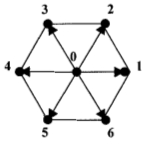
\includegraphics[width=0.3\textwidth]{img/fig1.png}
  \caption{The FHP hexagonal lattice [2].}
\end{figure}

There are many more different models of lattices. It is amazing that such discretization of the behavior of the particles can still lead to plausible simulation of hydrodynamics.

In such model the only think which we need to know is if there a particle in the vertex or not. The state of the lattice gas has a very small storage demand – 6N bits for N lattice sites.  Over the entire lattice the collection of occupation numbers $n_{i}(x,t)$ (n=0-particle absence, n=1-particle presence) defines an 6N-dimensional time-dependent Boolean field whose evolution happens in Boolean phase-space consisting of $2^{6N}$ discrete states.

We have already described different states in CA but in LGCA there are some extra evolution rules which are worth of consideration. Based on hydrodynamics we have such basic mechanisms:

\begin{itemize}
\item Free-streaming;
\item Collision.
\end{itemize}

Free-streaming is a simple transfer of particles according of their discrete velocities (see Fig. 2., 3.). The discrete free-streaming operator $\Delta i$ looks like this [2]:

\begin{equation}
\Delta_i n_i = n_i(x+c_{i}, t+1) - n_{i}(x,t)
\end{equation}

\begin{figure}[H]
  \centering
  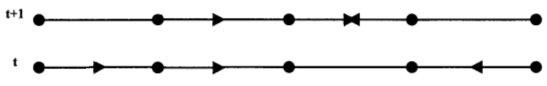
\includegraphics[width=0.7\textwidth]{img/fig2.png}
  \caption{Free-streamng in a discrete one-dimensional lattice [2].}
\end{figure}

\begin{figure}[H]
  \centering
  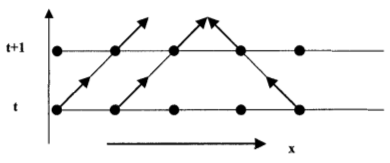
\includegraphics[width=0.5\textwidth]{img/fig3.png}
  \caption{Free-streaming along the light-cones of x-t space-time [2].}
\end{figure}

When two particles meet each other on the site they interact and exchange their momenta following the discretization rules of the lattice. Such exchange is called collision. In HPP only two particles can collide, that is why the collision in HPP is deterministic(see Fig. 4).

\begin{figure}[H]
  \centering
  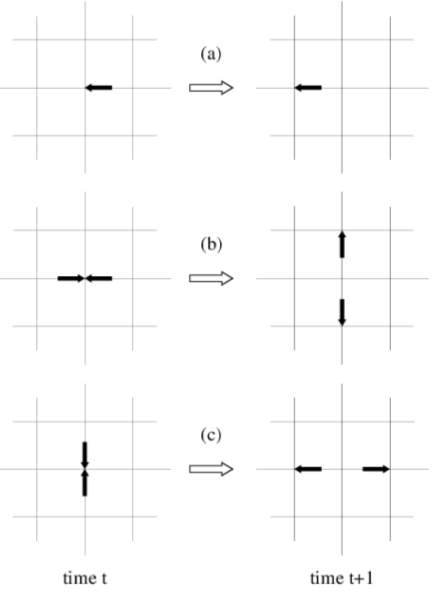
\includegraphics[width=0.5\textwidth]{img/fig4.png}
  \caption{A HPP collision of two particles.}
\end{figure}

If we will consider the collision of two particles in FHP, then we will have nondeterministic outcome(see Fig. 5).

\begin{figure}[H]
  \centering
  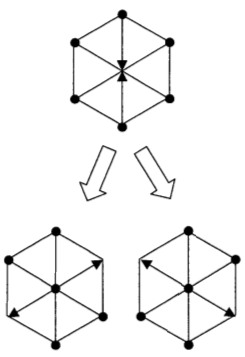
\includegraphics[width=0.5\textwidth]{img/fig5.png}
  \caption{A FHP collision with two equivalent outcomes [2].}
\end{figure}

Albeit all restrictions this collision shares two crucial features such as conversation of particle number and conversation of the total momentum.

\begin{itemize}
\item conserve mass (number of particles):
	\begin{equation}
\sum_i n_i^{in} = \sum_i n_i^{out}
	\end{equation}
\item onserve momentum:
	\begin{equation}
\sum_i n_i^{in} \overrightarrow{c}_{ia} = \sum_i n_i^{out} \overrightarrow{c}_{ia}
	\end{equation}
\end{itemize}

The exclusion principle is kept too. There are not two particles with the same position and velocity at the same time. The algorithm for simulation of hydrodynamics using LGCA looks like this:
while (t != t end ) \{
\begin{enumerate}
\item collide - handle multiple particles present at the same site 
\item stream - travel the respective edge 
\item $t = t + \Delta t $
\end{enumerate}
\}

Streaming: $ n_i^{in}(\overrightarrow{r}+\overrightarrow{c}_{i}\Delta t, t+\Delta t) = n_i^{out}(\overrightarrow{r}, t)$

Collision: $ n_i^{out}(\overrightarrow{r}, t) = n_i^{in}(\overrightarrow{r}, t) + \Omega(n_i^{in}(\overrightarrow{r}, t)) $

Where $\Omega$ is a collision operator. One of the biggest advantages of LGCA is it's easy implementation, and  the easiness of it's parallelization, because of locality of the update rule.

But the discretization works not always. For Macro-view such discretization is not a big problem, because we always discretize, but for Micro-view such restrictions can bring to huge inconsistency and very poor precision. Restriction in velocity direction and magnitude cannot describe model on microscopic level. In CA includes state of particle where the velocity is equal to zero(stationary particles), but in real word of microscopic level there can not exist such particles. There several main drawbacks of LGCA, but the most important one is statistical noise.

Lattice-Boltzmann approach was created as a respond on the main problems of LGCA, using an statistical averaging procedure.